%++++++++++++++++++++++++++++++++++++++++
% Don't modify this section unless you know what you're doing!
\documentclass[a4paper,11pt]{article}
\usepackage{listings} % code blocks
\usepackage{tabularx} % extra features for tabular environment
\usepackage{amsmath}  % improve math presentation
\usepackage{graphicx} % takes care of graphic including machinery
\usepackage{subcaption} % necessary for subfigures
\usepackage[margin=1.2cm,a4paper,nohead]{geometry} % decreases margins
\usepackage{cite} % takes care of citations
\usepackage[final]{hyperref} % adds hyper links inside the generated pdf file

%++++++++++++++++++++++++++++++++++++++++


\begin{document}

\title{First exercise: Classifying MNIST with MLPs}
\author{David-Elias K\"unstle}
\date{\today}
\pagenumbering{gobble} % turn of page numbering (not needed for 2 pages)
\maketitle
\section{Introduction}

In the following I report about my implementation and application of a multilayer perceptron
(MLP) for handwritten digit classification with the MNIST dataset.

I briefly describe my problems while implementation but focus more on
applying the MLP and an excursion to regularization, because for the former a
stricter course was already given.

\section{Implementation}

The implementation of the MLP was done according to the given framing, wherefore
I don't go into detail here.
The framing was only changed by moving some code to separate functions to
reuse, adding regularization (see \autoref{sec:regularization}) and
storing the error rate history while training for plotting.
Difficult was, that the parts of the MLP all depend on each other, such that
debugging can only be done by changing parts and checking \emph{does the
  error/loss decrease?} or \emph{are the gradients right?} (with gradient check).
Probably consequent test driven development with unit tests even for the layer
could help, but was not by myself.
Fortunately parts of MLP algorithm themself are simple, such that
they easily can be manually compared and verified to the formulas in text books
and slides.

I especially had difficulties with the gradient checker. Even after
verifying parts to work like \\ \texttt{scipy.optimize.check\_grad}
and a successfully learning network, the check failed.
In the end the gradient check still was useful, because it revealed
a mistake in the network implementation.
We divided the gradient by the number of samples in each layer,
which was not a problem for our 1 or 2 hidden-layer networks, but
would be for deeper.

\section{Application}

We use our implementation of a MLP to recognize (\emph{classify})
handwritten digits of the \emph{MNIST} dataset.
Setting up training of a MLP which does this classification with a very low
error rate in the end involves finding the right meta parameters.
We train, verify and test the network on separate datasets.
Meta parameters can be of the network (\emph{number of layers or hidden units,
  choice of activation functions}) or for training itself (\emph{learning rate,
  batch size, choice of optimization method, \dots}).
Training and verifying is time consuming, especially with huge datasets,
such we used a reduced training set with about 10000 items while searching for meta paramters.
Error rate is not exactly the same as with the full training set,
but we can see a tendency.
Still, training time is about one to three minutes on a \emph{Intel(R) Core(TM)
  i7-5600U CPU @ 2.60GHz}. Therefore meta parameter search was done manually
and very sparse.
Some parameter choices are obvious.
For gradient descent optimization is very difficult to
find a learning rate for which it learns but not overshoots. The stochastic
gradient descent (SGD) in contrast is way more robust even if it introduces the batch
size as another meta parameter.
More difficult is, that several meta parameters affect the error rate in a
coupled fashion.
It's annoying, if the loss does not decrease at all with the current meta parameters.
To at least get a point to start for further parameter tuning
I started with meta parameter combinations found in the exercise or internet
\cite{deeplearningorg}. Also first searching meta parameters like the learning rate
on logarithmic scale worked pretty well.

The setup in \autoref{fig:errorbest} is the one I ended up with.
Validation error converges after 15 epochs on the full MNIST training training
dataset (50000 images) to 1.7\%.
The test error on the unseen test dataset is 2.0\%.

\begin{figure}[ht]
  \centering 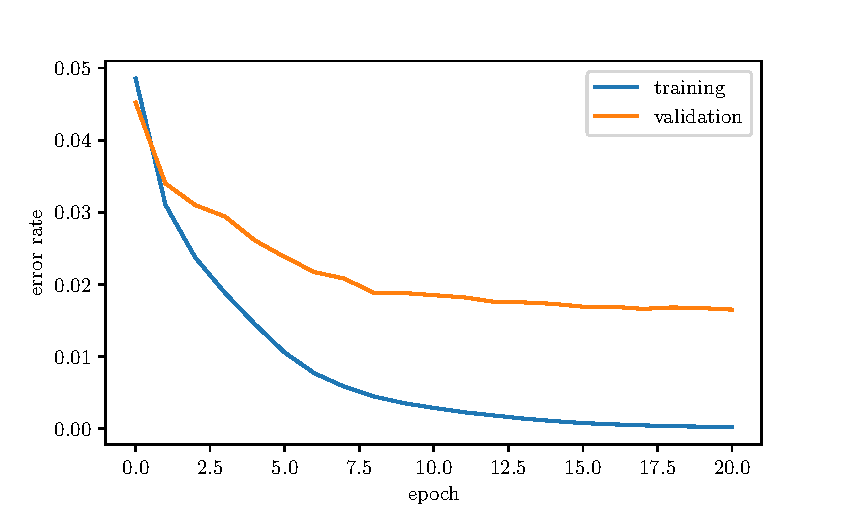
\includegraphics[width=0.55\textwidth]{assets/error_best.pdf}
  \caption{
    \label{fig:errorbest}
    Change of training and validation error while training epochs of MLP on full
    MNIST dataset. MLP has one hidden layer with 350 units and ReLu activation.
    Optimization with SGD used a learning rate of 0.4 and batches of 64 images.
  }
\end{figure}


\section{Regularization}\label{sec:regularization}

With the high amount of parameters (number of weight values), MLPs
are capable to express even complex functions.
This can lead to the problem of \emph{overfitting} which means the network
learns to express exactly the noisy training data instead of the general
underlying function. You see this generalization lack in \autoref{fig:errorbest}
as the gap between training and validation curves.
Regularization is an easy method to prevent overfitting by limiting the values
of the parameter vectors. Therefore I implemented
$L_1$ and $L_2$ regularization according to \cite{goodfellow71}.

$L_2$ regularization adds the squared sum of weights to the loss.
This means a large parameter values (huge square weight values) increase the loss a
lot and are therefore avoided. $L_1$ works similar but with the sum of absolute
parameter values. The amount of regularization can be controlled with the meta
parameter $\alpha$. In the regularization introduction in lecture we did set
$\alpha=\frac{2}{\#\theta}$.

\begin{align}
  L_{L_2}(f_\theta, D) &= L(f_\theta, D) + \frac{\alpha}{2} \theta^T \theta,
  &\theta \leftarrow \theta - \epsilon (\alpha \theta + \nabla_\theta L(f_\theta,
  D)) \\
  L_{L_1}(f_\theta, D) &= L(f_\theta, D) + \alpha \lVert \theta \rVert,
  &\theta \leftarrow \theta - \epsilon (\alpha \mathop{sign}(\theta) + \nabla_\theta L(f_\theta,D))
\end{align}

You see in \autoref{fig:errorreg} that - like expected - the validation and
training error rates are close.
Still also some draws of regularization are visible.
Both the train and the validation errors are higher with regularization.
Possibly this can be explained, by seeing the regularization update step also
as forgetting learned parameters.
In \autoref{fig:errorregl2} epochs 7 and 10 we see another incident which is
probably also caused by the forgetting. The error rates jump up before
descreasing again.

\begin{figure}
  \centering
  \begin{subfigure}[b]{0.3\textwidth}
    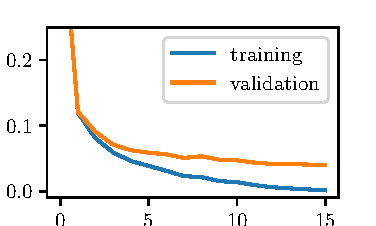
\includegraphics[width=\textwidth]{assets/error_noreg.pdf}
    \caption{none}
    \label{fig:errorregl1}
  \end{subfigure}
  \begin{subfigure}[b]{0.3\textwidth}
    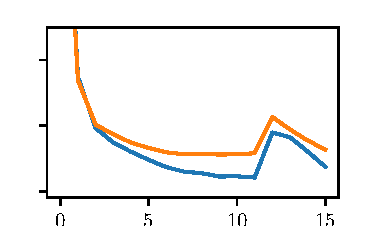
\includegraphics[width=\textwidth]{assets/error_l1.pdf}
    \caption{$L_1$ ($\alpha=0.0001$)}
    \label{fig:errorregl1}
  \end{subfigure}
  \begin{subfigure}[b]{0.3\textwidth}
    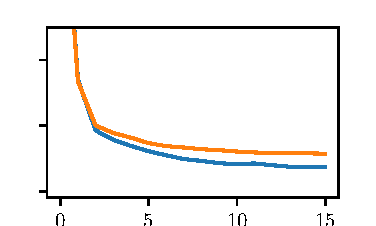
\includegraphics[width=\textwidth]{assets/error_l2.pdf}
    \caption{$L_2$  ($\alpha=0.005$)}
    \label{fig:errorregl2}
  \end{subfigure}
  \caption{Classification error while SGD training of MLP subset of MNIST without and with
    regularization. MLP has two hidden layers with each 100 units and ReLu activation.}\label{fig:errorreg}
\end{figure}



\begin{thebibliography}{99}
\bibitem{deeplearningorg}
  \url{http://deeplearning.net/tutorial/mlp.html}, last visit 2017/11/06
\bibitem{goodfellow71}
  I.\ Goodfellow, Y.\ Bengio, and A.\ Courville, \textit{Deep Learning, sec. 7.1},
  (MIT Press, 2016)
\end{thebibliography}

\end{document}
